\documentclass[12pt]{report}
\usepackage[utf8]{inputenc}
\usepackage[spanish,mexico]{babel}
\usepackage{apacite} % Paquetería para poder hacer referencias en APA
\usepackage{graphicx} % Paquete para poder añadir imagenes
\usepackage[letterpaper, margin=1in]{geometry}
\usepackage[T1]{fontenc}
\usepackage{tgbonum} % Cambia el tipo de letra
\usepackage{url}

\title{UNIVERSIDAD NACIONAL AUTÓNOMA DE MÉXICO\\ \ \\Facultad de Ingeniería\\ \ \\PROGRAMACIÓN ORIENTADA A OBJETOS\\ \ \\Proyecto 1 \\ \ \\Sistema de inscripciones \\}

\author{Carrichi de la Cruz, Roberto Carlos\\ \ \\Páez López, Didier Marcelo\\ \ \\Miranda Bueno, Fatima Yolanda \\ \ \\ \ \\ \ \\}
\date{Noviembre, 2020\\ \ \\Ciudad de México, México}

\begin{document}

\maketitle % Genera la portada del documento con los datos dados después de la declaración de paquetes


%--------------------------------------------------------------------
%---------------------------- ÍNDICE --------------------------------
%--------------------------------------------------------------------

\section*{Índice}
\begin{enumerate}
    \item Objetivos del proyecto \hfill 2
    \item Introducción
    \begin{enumerate}
        \item ¿Qué es una colección? \hfill 2
        \item Principales colecciones en Java \hfill 2
        \begin{enumerate}
            \item Set \hfill 3
            \item List \hfill 3
            \item Map \hfill 4
        \end{enumerate}
        \item Diferencias entre los tipos de colecciones \hfill 5
        \item ¿Cómo se establece la jerarquía de colecciones en Java? \hfill 5
        \item Factores a tomar en cuenta para la elección de \\una colección \hfill 6
    \end{enumerate}
    \item Desarrollo
    \begin{enumerate}
        \item Esctructura del sistema \hfill 7
        \item Elección de colecciones \hfill 7
        \item Características de cada clase utilizada \hfill 7
        \begin{enumerate}
            \item Proyecto \hfill 7
            \item Menu \hfill 8
            \item Alumno \hfill 8
            \item Asignatura \hfill 9
            \item Profesor \hfill 9
            \item Grupo \hfill 10
        \end{enumerate}
        \item Relaciones entre clases \hfill 11
    \end{enumerate}
    \item Conclusiones 
    \begin{enumerate}
        \item Conclusiones individuales \hfill 12
    \end{enumerate}
    \item Aclaraciones finales \hfill 12
    \item Referecias utilizadas \hfill 13
\end{enumerate}

\newpage % Crea un salto a la siguiente página

%----------------------------------------------------------------------
%--------------------- OBJETIVOS DEL PROYECTO -------------------------
%----------------------------------------------------------------------

\section*{Objetivos}

Que el alumno conozca los principales aspectos teóricos y prácticos de las colecciones y sus aplicaciones en el lenguaje de programación Java, así mismo que ponga en práctica los conceptos básicos de la programación orientada a objetos y el trabajo en equipo a distancia.

%--------------------------------------------------------------------
%------------------------- INTRODUCCIÓN -----------------------------
%--------------------------------------------------------------------

\section*{Introducción}
\subsubsection{¿Qué es una colección?}
Se le llaman colecciones a aquellas estructuras que representan un conjunto de objetos, siendo estos un tipo de dato abstracto con atributos y métodos capaces de manipular su propia información o la de otros objetos. \cite{Schildt}

%--------------------------------------------------------------------
\subsubsection{Principales colecciones en Java}
El objetivo de cada uno de estas estructuras fue proporcionar un alto rendimiento en cuanto a poder añadir, eliminar o cuantificar el contenido que tiene la colección, por otro lado, también son implementaciones que buscan hacer fácil poder extender y adaptar la información para que todas trabajen de forma similar, haciendo uso del polimorfismo, dado que tendrán los mismos métodos pero serán implementados de formas diferentes. \cite{Vindel} \\ Los métodos principales que tienen en común son los siguientes:\\

\begin{center}
    \begin{tabular}{|c|p{9cm}|}
        \hline
        Método& Función\\
        \hline\hline
        add( ) & Añadir elementos a la colección.\\
        \hline
        addAll( ) & Añadir todos los elementos de una colección a    otra.\\
        \hline
        remove( ) & Eliminar \textbf{un} elemento.\\
        \hline
        removeAll( ) & Eliminar un grupo de objetos.\\
        \hline
        retainAll( ) & Eliminar todos los elementos excepto un grupo específico.\\
        \hline
        clear( ) & Vaciar una colección.\\
        \hline
        contains( ) & Verificar si una colección tiene un objeto.\\
        \hline
        containsAll( ) & Determinar si una colección tiene todos los elementos de otra.\\
        \hline
        isEmpty( ) & Verificar si una colección se encuentra vacía.\\
        \hline
        size( ) & Obtener la cantidad de elementos que contiene la colección.\\
        \hline
        equals( ) & Para generar una comparación entre colecciones.\\
        \hline
    \end{tabular}    
\end{center}

\newpage
A continuación, se presentan las 3 de colecciones principales en el lenguaje Java. Cada una contiene características diferentes, pero solo 2 todas parten de las interfaces \textbf{Collection}, la cual presenta los métodos para una colección) y de \textbf{Iterator}, la que proporciona el medio para poder acceder a los elementos de una colección:

\subsubsection{Set}
Su principal característica es crear un conjunto de elementos en el cual \textbf{ninguno puede repetirse}. Por lo tanto, al utilizar el método add() primero se utilizará una verificación para saber si ya existe el valor en la colección. Se presenta al expresar: \textit{public interface Set<E> extends Coleccion<E>} y E especificará el tipo de objetos que el conjunto almacenará. \cite{ORACLE}
Sus principales implementaciones son:
\begin{itemize}
    \item HashSet \\ \\Hace referencia a una colección que utiliza una tabla de \textbf{dispersión} en la que serán almacenados los datos. La declaración de una colección de este tipo se realizará utilizando: \textit{class HashTable<E>} , expresando en el valor E el tipo de dato que contendrá la colección.
    \item LinkedHashSet\\ \\Es una clase que extiende el funcionamiento de HashSet la cuál \textbf{mantendrá el orden} en el que se añaden los elementos. La forma de declarar esta clase se hace así: \textit{class LinkedHashSet<E>}, inticando en E el tipo de valores que almacenará nuestra estructura. 
    \item TreeSet\\ \\ Hace uso de los atributos y métodos de la interfaz NavigableSet, generando así un árbol para el almacenamiento de datos. Una de sus ventajas es su velocidad en tiempos de acceso y recuperación de datos, los datos que se van añadiendo se mantienen en un orden ascendente. La instrucción para crear una instancia de este tipo se mantendrá la siguiente estructura: \textit{class TreeSet<E>}.
\end{itemize}

\subsubsection{List}
Esta interfaz define el comportamiento de una colección en la cual \textbf{sus elementos tienen una sucesión}. Aquí no importa si alguno de los elementos se repite. Para obtener un valor de esta lista se hará uso del método \textbf{get()} y \textbf{set()} para indicar un nuevo valor en una posición definida.\\ Aquí también se añadirán métodos de búsqueda con \textbf{intexOf} o \textbf{lastIndexOf} y de creación de sublistas con \textbf{subList()}, indicando el inicio y el final. Su estructura se presenta con: \textit{public interface List<E> extends Coleccion<E>} , donde E será el tipo de objetos que la lista va a contener.
Sus principales implementaciones son:
\begin{itemize}
    \item ArrayList\\ \\Su declaración está dada por: \textit{class ArrayList<E>}, colocando en E el tipo de dato que esta lista podrá almacenar. Es una clase que se dedica a soportar arreglos dinámicos que pueden incrementar o disminuir de tamaño según se requiera.
    \item LinkedList\\ \\ A diferencia de la otra implementación esta representa una lista doblemente ligada por. Su declaración está dada por: \textit{class LinkedList<E>} y el valor de E representará el tipo de valores que contendrá nuestra lista enlazada.
\end{itemize}

\subsubsection{Map}
Se dedica a ``mapear"\ \textbf{claves únicas de valores}, estas funcionarán como un elemento que ayudará a poder acceder a otro. Su forma de declaración estará dada por: public interface Map<K,V> , en la cual el valor de K representará el tipo de las \textbf{claves} y V el tipo de \textbf{valores}. \cite{Departament}
Sus principales implementaciones son:
\begin{itemize}
    \item HashMap: Esta implementación hace uso de una tabla de dispersión para almacenar información de referencias de datos, con el fin de crear \textbf{búsquedas muy eficientes} de velocidad constante al utilizar su método get(). Para crear una estructura de este tipo se utiliza la instrucción: \textit{class HashMap <K,V>}.
    
    \item TreeMap: Aquí se hace uso de una estructura de árbol, lo cual hace muy eficiente el proceso de añadir datos a la colección, a diferencia de las tablas de dispersión, esta estructura asegura mantener un orden en sus elementos de forma ascendente. Para implementarlo se expresa así: \textit{class TreeMap <K,V>}, con el valor K se especifica el tipo de clave y con el valor V el tipo de valores que contendrá la estructura.
    
    \item LinkedHashMap: Su funcionamiento tiene mucha relación a la estructura HashMap, solo que en esta se mantiene una lista enlazada de las entradas al mapa y se \textbf{mantiene el orden en que fueron insertadas}, haciendo posible poder hacer un recorrido dentro de la escructura para alguna iteración que necesitemos. Para declarar una instancia se utiliza: \textit{class LinkedHashMap<K,V>}, siguiendo la misma estructura de los valores K y V como lo hacemos en HashMap. 
\end{itemize}

%--------------------------------------------------------------------
\subsubsection{Diferencias entre los tipos de colecciones}
\begin{center}
    \begin{tabular}{||p{4cm}|p{3cm}|p{3cm}|p{3cm}||}
        \hline
        &Set & List & Map \\
         \hline\hline
        Repetición de datos:&No permite.&Si permite.&Si permite.\\
         \hline
        Mantiene orden en su contenido:&No mantiene orden.&Si mantiene el orden.&No tiene mantiene orden.\\
         \hline
        Es derivado de la clase Coleccion&Sí es derivado.&Sí es derivado. &No es derivado.\\
         \hline
        Implementaciones:&HashSet, LinkedHashSet, TreeSet &ArrayList, LinkedList&HashTable, HashMap, LinkedHashMap, TreeMap\\
         \hline
        \end{tabular}
\end{center}

%-------------------------------------------------------------------
\subsubsection{¿Cómo se establece la jerarquía de colecciones en Java?}
\begin{enumerate}
    \item De la interfaz Collection parten \textbf{la mayoría de las colecciones}.
    \item Existirán tres grandes interfaces que son las principales en todas las colecciones, dos de ellas son descendientes de Collection, estas son: \textbf{Set, List}. La interfaz \textbf{Map} estará denominada como una interfaz intependiente, ya que en esta se establecen métodos diferentes a comparación de las otras dos interfaces.
    
    \item De la interfaz Set se generarán otras dos ramificaciones, de las cuales una de ellas es una implementación directa llamada \textbf{HashSet} (la cual será la clase padre de \textbf{LinkedHashSet}), en la otra ramificación encontraremos dos interfaces: SortedSet y NavigableSet, las cuales serán la base para crear la clase \textbf{TreeSet}.
    
    \item Por parte de la interfaz List, existirán dos implementaciones directass: \textbf{ArrayList} y \textbf{LinkedList}.
    
    \item Mediante la interfaz Map, podrémos encontrar 2 implementaciones directas (\textbf{HashTable} y \textbf{HashMap}, esta última tendrá la clase derivada \textbf{LinkedHashMap}) y una interfaz derivada llamada SortedMap, la cual junto con su interfaz derivaba NavigableMap generarán la colección de tipo \textbf{TreeMap}.
\end{enumerate}
\begin{center}
    \includegraphics[width=0.9\textwidth]{img/Jerarquía de colecciones.png}\\ \ \\Diagrama basado en el propuesto por: \cite{Colecciones}
\end{center}



%--------------------------------------------------------------------
\subsubsection{Factores a tomar en cuenta para la elección de una colección}
De acuerdo a las características proporcionadas anteriormente, la forma de elegir la mejor estructura según nuestras necesidades se llevará en un orden determinado de condiciones.
\begin{enumerate}
    \item Establecer los tipos de valores que se utilizarán, \textbf{¿serán de clave-valor?}
    \item Definir el cómo serán utilizados los datos, \textbf{¿se podrán repetir?}
    \item Determinar si en necesario que lleven una estructura definida, \textbf{¿los datos deben estar ordenados?}
    \item Por último, en dado caso que si deben estar acomodados, \textbf{¿se ordenarán siguiendo el orden en que entran o en orden de acuerdo a sus claves?}
\end{enumerate}

\begin{center}
    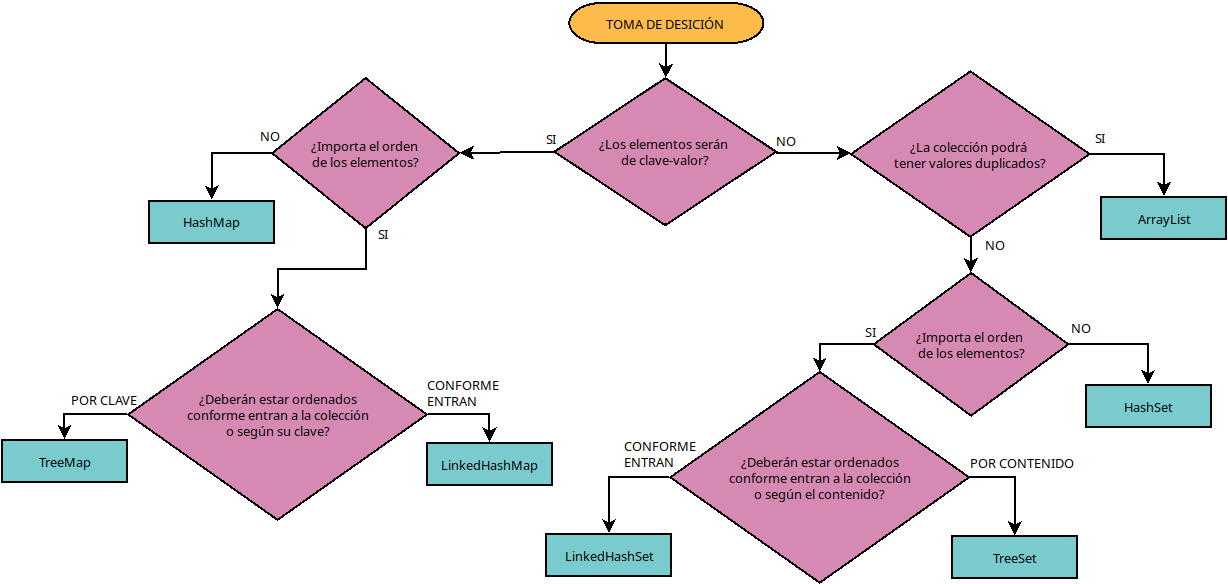
\includegraphics[width=0.9\textwidth]{img/Elección de una colección.png}
\end{center}


%--------------------------------------------------------------------
%------------------- DESARROLLO DEL PROYECTO ------------------------
%--------------------------------------------------------------------

\section*{Desarrollo}

\subsubsection{Estructura del sistema}
Este programa, que tiene como propósito simular un sistema de inscripciones para alumnos, profesores, asignaturas y grupos, se divide en seis clases: Proyecto, Menu, Alumno,Asignatura, Grupo y Profesor.\\
En las primeras dos clases se hace la elección de la actividad a realizar por el usuario. En las restantes clases se añaden objetos, se muestran los atributos de los objetos y se realiza la composición de clases.

%begin{itemize}
 %   \item Estructura del sistema
    
%\end{itemize}

%--------------------------------------------------------------------

\subsubsection{Elección de colecciones}
Como se mencionó en la sección incluida en la introducción \textit{Factores a tomar en cuenta para la eleccion de una coelccion}, la forma de seleccionar el tipo de colección a utilizar y la implementación que utiliza Java para cada una, se puede realizar analizando los requerimientos solicitados.\\
En la clase Alumno, se decidió utilizar una lista de alumnos, más específicamente, se utilizó la interfaz List , la clase Arraylist, la cual proporciona la implementación de un arreglo dinámico. Esta elección se realizó debido a que, aunque en principio no deberían de existir elementos o valores duplicados (es decir, alumnos duplicados), su tarea principal será almacenar y buscar los objetos almacenados en esta colección, que sus uso será más evidente en la clase Grupo, la cual se analizará a detalle en la sección e). \\
El mismo razonamiento para la toma de decisión anterior con la colección para Alumno, se realizó para las clases de Asignatura y Profesor, ya que su principal función será almacenar objetos de estos tipos, implementando un arreglo dinámico.\\
Este tipo de colecciones son dinámicas, por lo que no existe un límite en la cantidad de alumnos, asignaturas o profesores por inscribir.\\
Otro tipo de colección utilizada fue Enumeration para Integer, sin embargo este no es ningún atributo, es una variable del método inscritos() dentro de la clase Grupo. En este se guardan las claves de los grupos de la lista HasTable, y se utiliza como la implementación de una estructura queue.

%\begin{itemize}
 %   \item Elección de colecciones
%\end{itemize}




%--------------------------------------------------------------------


\subsubsection{Características de cada clase utilizada}
En esta sección se describirán los atributos y métodos que conforman cada clase, así como su funcionalidad básica con un cierto nivel de abstracción.
\begin{itemize}
\item Proyecto \\ \\
Por la clase que iniciamos sera Proyecto, dentro de la cual se encuentra el método main, por lo que sera donde inicia este programa y manda a llamar a las demás clases y sus métodos (su relación se decribirá en la siguiente sección d) ). Esta clase no cuenta con ningún atributo. El único método, como se mencionó antes, es main(), en el cual se manipulan las elecciones de las opciones a realizar por el usuario y con estructuras switch, llamar a los métodos correspondientes de las demás clases (para lo cual es necesario crear objetos de estas).\\
Cabe resaltar que no es parte de ningún paquete, ni se importa ninguna clase o método específico, ya que las entradas de datos se darán a través de las otras clases.\\

\item Menu \\ \\
En esta clase se encuentran los menú para que el usuario seleccione una opción a realizar. De igual manera, esta clase no cuenta con atributos. Cuenta con dos métodos, ambos con el propósito de oprimidos tipo de menú y de regresar la opción tomada, por esta razón la única clase que se importa a la clase es Scanner.\\



\item Alumno\\ \\
Esta clase es la encargada de gestionar los métodos y atributos que corresponden a un alumno.\\
Los atributos con los que cuenta esta clase son las características que se toman para un alumno, tales como nombre (nombre de pila y apellido), número de cuenta y el semestre; además de estos, otro atributo es una lista de alumnos, llamada “alumnitos” (la misma clase) donde se registraron todos los objetos creados de este tipo, y una variable estática que lleva la cuenta de todos los alumnos.\\
En la clase se incluyen los siguientes tipos de métodos:
\begin{itemize}
    \item Constructores: uno vacío, y otro donde se asignan los valores de los tres atributos característicos.
    \item registrarAlumno() en el cual se solicita al usuario los datos de cada alumno a ingresar a la lista de Alumno.
    \item info() muestra los atributos característicos del alumno que utiliza el método.
    \item imprimirAlumnos(): muestra los atributos de todos los objetos de tipo Alumno en la lista alumnitos, con ayuda del método anterior info().
    \end{itemize}
Esta clase importa las clases Scanner y ArrayList.
\newpage
\item Asignatura \\ \\ 
En esta clase se gestiona los métodos y atributos que se consideran necesarios para una asignatura.\\
Dentro de los atributos de la clase se encuentra el nombre de la asignatura, los créditos correspondientes y las horas a la semana correspondientes; igual que en la clase Alumno, se incluye un atributo el cual es una lista de objetos de tipo Asignatura, llamada “materias”; y por último una variable estática que cuenta la cantidad de asignaturas registradas.\\
Esta clase contiene los siguientes métodos:
\begin{itemize}
\item Constructores: uno vacío y otro con los atributos de nombre, créditos y horas, además aumenta el número de asignaturas registradas.
\item registrarAsignatura(): en este método se añaden a la lista los valores para los atributos ingresados por el usuario.
\item info(): muestra los atributos del objeto (Asignatura) que utiliza este método.
\item mostrarAsignaturas(): Con este método y del anterior se imprimen todas las asignaturas dentro de la lista “materias”.
\end{itemize}
Las clases que importa son ArrayList y Scanner.\\


\item Profesor \\ \\
Con esta clase se gestionan los atributos y los métodos para construir un objeto de tipo Profesor.\\
Esta clase cuenta con los atributos de nombre del profesor, título del profesor y los años que lleva impartiendo clase; así como una lista que almacena objetos de tipo Profesor, llamada “maestros”; y un contador de la cantidad de profesores registrados por el sistema.\\
La clase Profesor cuenta con los siguientes métodos.
\begin{itemize}
\item  Constructores: uno vacío y otro donde se ingresan los atributos antes mencionados, sin contar la lista, y se incrementa el total de profesores registrados.
\item registrarProfesor(): esta clase solicite al usuario ingresar los datos del profesor a registrar y añade el objeto a la lista de Profesores.
\item info(): este método imprime los valores de los atributos del objeto tipo Profesor que manda a llamar al método.
\item imprimirProfesor(): imprime los valores de los atributos de todos los objetos dentro de la lista “maestros”.
\end{itemize}
Igual que en las clases anteriores, esta importa ArrayList y Scanner.
\\

\item Grupo  \\ \\
esta probablemente sea la clase mas compleja del programa, ya que es la que hace la composición o relación entre clases.\\
Los atributos de esta clase son la clave del grupo; las listas de las clases anteriores (Grupo, Asignatura y Profesor); un contador que registra cada que se crea un nuevo grupo; y la implementación de una Hashtable, que tiene como llaves la clave del grupo y como valor la lista de alumnos inscritos en dicho grupo, esta se llama “lista”.\\
\\Los métodos de la clase son los siguientes:
\begin{itemize}
\item constructores: uno vacío y otro con la clave como parámetro, además de incrementar el contador de grupos.
\item abrirGrupo(): en este método el usuario elige, entre la lista de profesores y de asignaturas existentes, con cuales abrirá un nuevo grupo. Además, confirma en la lista de grupos que la clave ingresada no esté repetida. Si no es el caso entonces asigna un grupo, el profesor y la asignatura, junto con la clave, a la lista de grupos.
\item lista profesores(): este método se utiliza como auxiliar en el método anterior, e imprime la lista de objetos Profesor registrados en la lista profesores.
\item listaAsignaturas(): como en el metodo anterior, este imprime todos los objetos de tipo Asignatura registrados en la lista materias.
\item asignarA(): otro método que se utiliza como auxiliar en el método abrirGrupo(), es la que busca si la asignatura que se quiere para un grupo se encuentra registrada en la lista de asignaturas, si sí regresa el objeto, si no, regresa valores nulos.
\item asignarP(): este método tiene el mismo propósito que el anterior, con la diferencia de que lo que busca es coincidencia entre el profesor deseado y la lista de profesores.
\item mostrarGrupos(): recorre la lista que contiene a todos los grupos registrados, e imprime cada uno de estos, con su profesor, asignatura y clave.
\item inscribirAlumnos(): en este método es donde se da la composición de clases. Dada la lista de los grupos abiertos y de los alumnos ya registrados en el sistema, el usuario debe escoger uno de cada uno; si el grupo ya se ha creado un grupo con alumnos, entonces se verifica si el alumno por inscribir ya está o no; si el grupo aún no cuenta con alumnos inscritos entonces se agrega dicho grupo con su primer alumno a la lista hashtable.
\newpage
\item imprimirClaves(): este método se ocupa en inscribirAlumnos, con el propósito de mostrarle al usuario las claves de los grupos existentes.
\item alumnosRegistrados(): de igual manera se utiliza en el método incribirAlumnos() para mostrar los alumnos registrados y sus números de cuenta, así el usuario podrá elegir uno.
\item selecGrupo(): este método también se utiliza en inscribirAlumnos(), y este se repite mientras el usuario no ingrese un grupo ya registrado, por lo que garantiza que se elija uno.
\item selecAlu(): este tiene el mismo propósito que el anterior, pero para objetos de tipo Alumno, mientras no coincida el ingresado con alguno registrado, se regresará un valor nulo y se repite.
\item inscritos(): este método se llama justo después del método mostrarGrupos(), ya que muestra para cada grupo dentro de la lista HashTable todos los alumnos inscritos de dicho grupo.

\end{itemize}

%\begin{itemize}
 %   \item Características de cada clase utilizada
%\end{itemize}




%--------------------------------------------------------------------


\subsubsection{Relaciones entre clases}
Como se mencionó en el punto anterior, la composición o relación entre las clases Alumno, Asignatura y Profesor, se da en la clase Grupo. Esta clase cuenta con listas de cada una de las clases mencionadas, además de la implementación de HashTable, para relacionar conjuntos de alumnos con el grupo al que pertenecen.\\
La primera relación en dicha clase surge en el método abrirGrupo, ya que relaciona a un objeto tipo Profesor de la lista de profesores registrados con un objeto de tipo Asignatura de la lista de materias registradas , el resultado es un objeto de tipo Grupo que se añade a la lista “grupitos”. Cabe resaltar que las listas que utiliza son las creadas en las clases Asignatura y Profesor, mas no los atributos de Grupos (listas “asignaturas” y “profes”), que guardan los objetos de tipo Asignatura y Profesor que forman en un objeto de tipo Grupo (estos se pueden repetir, lo que no se puede repetir es la clave de cada grupo).\\
El otro método que relaciona objetos de diferentes clases es inscribirAlumnos, ya que dada la lista de alumnos registrados en el sistema (en la lista “alumnitos”) y los grupos creados en el método anterior (que es un atributo de esta clase), ingresa en la Hashtable “lista” (donde las llaves son las claves de los grupos -números enteros- y los valores son la lista de alumnos que están inscritos en este grupo) el atributo clave de Grupo con objetos de tipo alumno, y como es una lista puede haber más de uno pero no se pueden repetir.\\



\end{itemize}
%--------------------------------------------------------------------

\newpage
%--------------------------------------------------------------------
%------------------ CONCLUSIONES DEL PROYECTO -----------------------
%--------------------------------------------------------------------
\section*{Conclusiones individuales}

\begin{itemize}
    \item Carrichi de la Cruz, Roberto Carlos
\end{itemize}
%Escribe tu conclusión a partir de aquí
El desarrollo de este proyecto resultó de mucha utilidad para conocer en profundidad los aspectos teóricos y prácticos de estructuras más complejas como lo son las colecciones, asimismo, hacer uso de estas nos da la capacidad de hacer programas más completos y al mismo tiempo hacen más eficaz el manejo de información. Por otro lado, fue muy positivo poder trabajar en equipo para la realización del proyecto, ya que gracias a esto se conocieron nuevas herramientas para el trabajo colaborativo como en el caso de GitHub para mantener la información actualizada en dispositivos remotos y Overleaf para la creación de archivos de LaTeX de forma colaborativa.

\begin{itemize}
    \item Páez López, Didier Marcelo
\end{itemize}    
%Escribe tu conclusión a partir de aquí
El uso de colecciones en la resolución de problemas de informática son una herramienta que resulta de gran ayuda, para saber cual es la colección más adecuada para implementarla y solucione el problema de la manera más efectiva en primer lugar hay que hacer un análisis previo del problema, con la visión general de la resolución de este podremos saber cuál será la colección que en ese caso será la más adecuada para la resolución del problema.

La aplicación del paradigma orientada a objetos y la aplicación de colecciones como los métodos de las mismas durante la resolución del proyecto fueron parte fundamental del mismo, ya que implementarlas fueron la base para poder hacer que el programa funcionara, los objetivos se cumplieron con éxito ya que básicamente en todo el programa se aplicó el paradigma y a pesar de haber sido a distancia la organización tanto individual como en equipo fue correcta para culminar el proyecto de manera acertada a los requerimientos iniciales.

\begin{itemize}
    \item Miranda Bueno, Fatima Yolanda
\end{itemize}
%Escribe tu conclusión a partir de aquí
Para la elaboración de este proyecto se requirió de la comprensión de los tipos de colecciones, las interfaces, las clases que los implementa y los métodos que Java proporciona. El crear este programa ayudó  a la comprensión de los casos en los que se debe de utilizar una u otra implementación de las colecciones, teniendo en cuenta los requerimientos del mismo programa. Asimismo cabe mencionar que un objetivo adicional en la elaboración de este proyecto (fuera de los relacionados con conceptos de programación) fue el resolver un problema planteado en equipo, desde la estructura que se daría al programa, hasta el enfoque que se tendría en la investigación; sin mencionar el reto del trabajo a distancia.

\section*{Aclaraciones finales}
\begin{itemize}
    \item Para un mejor entendimiento de los diagramas propuestos, se recomienda abrir la imagen directamente desde un sistema de archivos que soporte el formato .png, .jpeg y sus derivados. Estos se encuentran disponibles a la fecha en que se presenta este documento.
    \item Si es requerido el código del proyecto para tener una mejor comprensión, puede encontrar en el siguiente repositorio de GitHub la última versión de los archivos fuente y la documentación correspondiente:  
    \begin{center}
        \url{https://github.com/RobertoCarrichi/POO_Proyecto_1_Equipo_12}
    \end{center}
\end{itemize}

%--------------------------------------------------------------------
%-------------------- REFERENCIAS UTILIZADAS ------------------------
%--------------------------------------------------------------------

% Etiquetas que crean la sección de las referencias que utilizamos con el formato APA

\bibliographystyle{apacite}

\bibliography{referencias.bib}

\end{document}
